\hypertarget{example-2.6-20-network-problem}{%
\section{EXAMPLE 2.6-20 \{Network
Problem)}\label{example-2.6-20-network-problem}}

Given below is a network in which the figures written against the arrows
(links) indicate the cost of travelling in rupees from the preceding to
the following node.

\begin{figure}
\centering
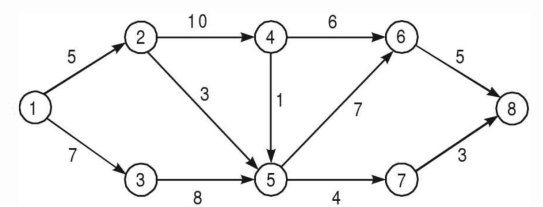
\includegraphics{figs/example_2-06-20.png}
\caption{Netework}
\end{figure}

Formulate the linear programming model to find the least cost route from
node 1 to node 8.
